%%%%%%%% ICML 2023 EXAMPLE LATEX SUBMISSION FILE %%%%%%%%%%%%%%%%%

\documentclass{article}

\usepackage[font=footnotesize,labelformat=simple]{subcaption}
\usepackage{tikz}
%\usepackage{etoolbox} % for \ifthen
\usepackage{listofitems} % for \readlist to create arrays
\usetikzlibrary{arrows.meta} % for arrow size
\usepackage[outline]{contour} % glow around text
\contourlength{1.4pt}

\tikzset{>=latex} % for LaTeX arrow head
\usepackage{xcolor}
\colorlet{myred}{red!80!black}
\colorlet{myblue}{blue!80!black}
\colorlet{mygreen}{green!60!black}
\colorlet{myorange}{orange!70!red!60!black}
\colorlet{mydarkred}{red!30!black}
\colorlet{mydarkblue}{blue!40!black}
\colorlet{mydarkgreen}{green!30!black}
\tikzstyle{node}=[thick,circle,draw=myblue,minimum size=22,inner sep=0.5,outer sep=0.6]
\tikzstyle{node in}=[node,green!20!black,draw=mygreen!30!black,fill=mygreen!25]
\tikzstyle{node hidden}=[node,blue!20!black,draw=myblue!30!black,fill=myblue!20]
\tikzstyle{node convol}=[node,orange!20!black,draw=myorange!30!black,fill=myorange!20]
\tikzstyle{node out}=[node,red!20!black,draw=myred!30!black,fill=myred!20]
\tikzstyle{connect}=[thick,mydarkblue] %,line cap=round
\tikzstyle{connect arrow}=[-{Latex[length=4,width=3.5]},thick,mydarkblue,shorten <=0.5,shorten >=1]
\tikzset{ % node styles, numbered for easy mapping with \nstyle
  node 1/.style={node in},
  node 2/.style={node hidden},
  node 3/.style={node out},
}
\def\nstyle{int(\lay<\Nnodlen?min(2,\lay):3)} % map layer number onto 1, 2, or 3
% Recommended, but optional, packages for figures and better typesetting:
\usepackage{microtype}
\usepackage{graphicx}
% \usepackage{subfigure}
\usepackage{booktabs} % for professional tables

% hyperref makes hyperlinks in the resulting PDF.
% If your build breaks (sometimes temporarily if a hyperlink spans a page)
% please comment out the following usepackage line and replace
% \usepackage{icml2023} with \usepackage[nohyperref]{icml2023} above.
\usepackage{hyperref}


% Attempt to make hyperref and algorithmic work together better:
\newcommand{\theHalgorithm}{\arabic{algorithm}}

% Use the following line for the initial blind version submitted for review:
\usepackage[accepted]{icml2023}

% If accepted, instead use the following line for the camera-ready submission:
% \usepackage[accepted]{icml2023}

% For theorems and such
\usepackage{amsmath}
\usepackage{amssymb}
\usepackage{mathtools}
\usepackage{amsthm}

% if you use cleveref..
\usepackage[capitalize,noabbrev]{cleveref}

%%%%%%%%%%%%%%%%%%%%%%%%%%%%%%%%
% THEOREMS
%%%%%%%%%%%%%%%%%%%%%%%%%%%%%%%%
\theoremstyle{plain}
\newtheorem{theorem}{Theorem}[section]
\newtheorem{proposition}[theorem]{Proposition}
\newtheorem{lemma}[theorem]{Lemma}
\newtheorem{corollary}[theorem]{Corollary}
\theoremstyle{definition}
\newtheorem{definition}[theorem]{Definition}
\newtheorem{assumption}[theorem]{Assumption}
\theoremstyle{remark}
\newtheorem{remark}[theorem]{Remark}

% Todonotes is useful during development; simply uncomment the next line
%    and comment out the line below the next line to turn off comments
%\usepackage[disable,textsize=tiny]{todonotes}
\usepackage[textsize=tiny]{todonotes}


% FIGURE DEFINITIONS
\newcommand*{\selfattentiongraph}{
    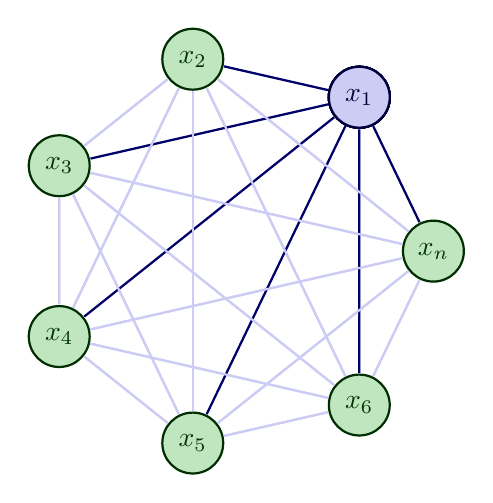
\begin{tikzpicture}
      \def\yshift{0.4} % shift last node for dots
      \def\xshift{0.4} % shift last node for dots
    
      \def\NI{7} % number of nodes in input layers
    
        % DRAW NODES
        \foreach \j [evaluate={\indexj=(\j<\NI?int(\j):"n");}] in {1,...,\NI}{
                \node[node in] (NI-\j) at (360/\NI * \j:2.5cm) {$x_{\indexj}$};
                % \draw[connect, myblue!100] (NI-\j) -- (NI-\i);
                % \draw[connect] (NI-\j) -- (NO-\i)
            }
        % DRAW EDGES
        \foreach \j [evaluate={\indexj=(\j<\NI?int(\j):"n");}] in {1,...,\NI}{
    
            \foreach \i [evaluate={\indexi=(\i<\NI?int(\i):"n");}] in {1,...,\NI}{     
                % \draw[connect, myblue!20] (NI-\j) -- (NI-\i);
                \ifnum\i=1 % high-lighted node
                    \node[node hidden] (NO-\i) at (360/\NI * \i:2.5cm) {$x_{\i}$};
                    \draw[connect] (NI-\j) -- (NI-\i);
                \else
                    \draw[connect, myblue!20] (NI-\j) -- (NI-\i);
                \fi
            }
        }
      % % DOTS
      % \path (NI-\NI) --++ (\xshift,1+\yshift) node[midway,scale=1.2] {$\vdots$};
    \end{tikzpicture}
}


\newcommand*{\crossattentiongraph}{

    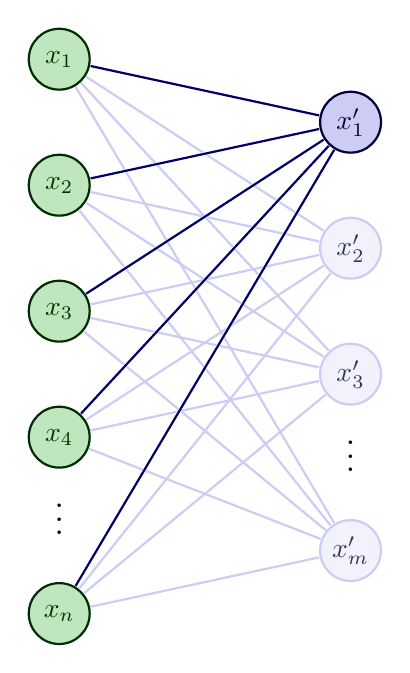
\begin{tikzpicture}[x=3.7cm,y=1.6cm]
      \def\NI{5} % number of nodes in input layers
      \def\NO{4} % number of nodes in output layers
      \def\yshift{0.4} % shift last node for dots
      
      % INPUT LAYER
      \foreach \i [evaluate={\c=int(\i==\NI); \y=\NI/2-\i-\c*\yshift; \index=(\i<\NI?int(\i):"n");}]
                  in {1,...,\NI}{ % loop over nodes
        \node[node in,outer sep=0.6] (NI-\i) at (0,\y) {$x_{\index}$};
      }
      % OUTPUT LAYER
      \foreach \i [evaluate={\c=int(\i==\NO); \y=\NO/2-\i-\c*\yshift; \index=(\i<\NO?int(\i):"m");}]
        in {\NO,...,1}{ % loop over nodes
        \ifnum\i=1 % high-lighted node
          \node[node hidden]
            (NO-\i) at (1,\y) {$x_{\index}'$};
          \foreach \j [evaluate={\index=(\j<\NI?int(\j):"n");}] in {1,...,\NI}{ % loop over nodes in previous layer
            \draw[connect,white,line width=1.2] (NI-\j) -- (NO-\i);
            \draw[connect] (NI-\j) -- (NO-\i)
              node[pos=0.50] {\contour{white}{}};
          }
        \else % other light-colored nodes
          \node[node,blue!20!black!80,draw=myblue!20,fill=myblue!5]
            (NO-\i) at (1,\y) {$x_{\index}'$};
          \foreach \j in {1,...,\NI}{ % loop over nodes in previous layer
            % \draw[connect,white,line width=1.2] (NI-\j) -- (NO-\i);
            \draw[connect,myblue!20] (NI-\j) -- (NO-\i);
          }
        \fi
      }
      
      % DOTS
      \path (NI-\NI) --++ (0,1+\yshift) node[midway,scale=1.2] {$\vdots$};
      \path (NO-\NO) --++ (0,1+\yshift) node[midway,scale=1.2] {$\vdots$};
    \end{tikzpicture}
}


\newcommand*{\mchngraph}{

    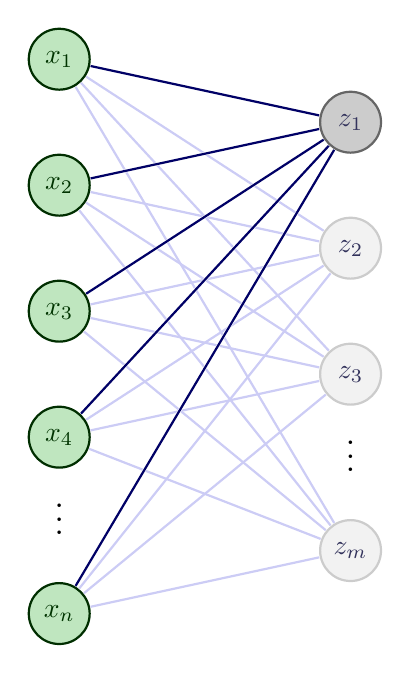
\begin{tikzpicture}[x=3.7cm,y=1.6cm]
    % MCHN
      \def\NI{5} % number of nodes in input layers
      \def\NO{4} % number of nodes in output layers
      \def\yshift{0.4} % shift last node for dots
      
      % INPUT LAYER
      \foreach \i [evaluate={\c=int(\i==\NI); \y=\NI/2-\i-\c*\yshift; \index=(\i<\NI?int(\i):"n");}]
                  in {1,...,\NI}{ % loop over nodes
        \node[node in,outer sep=0.6] (NI-\i) at (0,\y) {$x_{\index}$};
      }
      % OUTPUT LAYER
      \foreach \i [evaluate={\c=int(\i==\NO); \y=\NO/2-\i-\c*\yshift; \index=(\i<\NO?int(\i):"m");}]
        in {\NO,...,1}{ % loop over nodes
        \ifnum\i=1 % high-lighted node
          \node[node,blue!20!black!80,draw=black!60,fill=black!20]
            (NO-\i) at (1,\y) {$z_{\index}$};
          \foreach \j [evaluate={\index=(\j<\NI?int(\j):"n");}] in {1,...,\NI}{ % loop over nodes in previous layer
            \draw[connect,white,line width=1.2] (NI-\j) -- (NO-\i);
            \draw[connect] (NI-\j) -- (NO-\i)
              node[pos=0.50] {\contour{white}{}};
          }
        \else % other light-colored nodes
          \node[node,blue!20!black!80,draw=black!20,fill=black!5]
            (NO-\i) at (1,\y) {$z_{\index}$};
          \foreach \j in {1,...,\NI}{ % loop over nodes in previous layer
            % \draw[connect,white,line width=1.2] (NI-\j) -- (NO-\i);
            \draw[connect,myblue!20] (NI-\j) -- (NO-\i);
          }
        \fi
      }
      
      % DOTS
      \path (NI-\NI) --++ (0,1+\yshift) node[midway,scale=1.2] {$\vdots$};
      \path (NO-\NO) --++ (0,1+\yshift) node[midway,scale=1.2] {$\vdots$};
    \end{tikzpicture}
}


\newcommand*{\slotattentiongraph}{

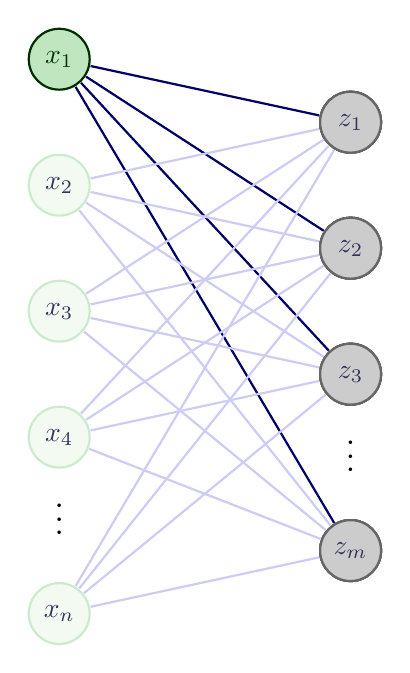
\begin{tikzpicture}[x=3.7cm,y=1.6cm]
% SLOT  
      \def\NI{5} % number of nodes in input layers
      \def\NO{4} % number of nodes in output layers
      \def\yshift{0.4} % shift last node for dots
      
      % INPUT LAYER
      \foreach \i [evaluate={\c=int(\i==\NI); \y=\NI/2-\i-\c*\yshift; \index=(\i<\NI?int(\i):"n");}]
                  in {1,...,\NI}{ % loop over nodes
        \ifnum\i=1 % high-lighted node
            \node[node in,outer sep=0.6] (NI-\i) at (0,\y) {$x_{\index}$};
        \else
            \node[node,blue!20!black!80,draw=mygreen!20,fill=mygreen!5] (NI-\i) at (0,\y) {$x_{\index}$};
        \fi
      }
      % OUTPUT LAYER
      \foreach \i [evaluate={\c=int(\i==\NO); \y=\NO/2-\i-\c*\yshift; \indexi=(\i<\NO?int(\i):"m");}] in {\NO,...,1}{ % loop over nodes
              \foreach \j [evaluate={\indexK=(\j<\NI?int(\j):"n");}] in {1,...,\NI}{ % loop over nodes in previous layer
                    \node[node,blue!20!black!80,draw=black!60,fill=black!20]
                (NO-\i) at (1,\y) {$z_{\indexi}$};
            \ifnum\j=1 % high-lighted node
                \draw[connect,white,line width=1.2] (NI-\j) -- (NO-\i);
                \draw[connect] (NI-\j) -- (NO-\i);
                  node[pos=0.50] {\contour{white}{}};
            \else % other light-colored nodes
                % \draw[connect,white,line width=1.2] (NI-\j) -- (NO-\i);
                \draw[connect,myblue!20] (NI-\j) -- (NO-\i);
        \fi
        }
      }
      
      % DOTS
      \path (NI-\NI) --++ (0,1+\yshift) node[midway,scale=1.2] {$\vdots$};
      \path (NO-\NO) --++ (0,1+\yshift) node[midway,scale=1.2] {$\vdots$};
    \end{tikzpicture}
}


\newcommand*{\blockslotattentiongraph}{

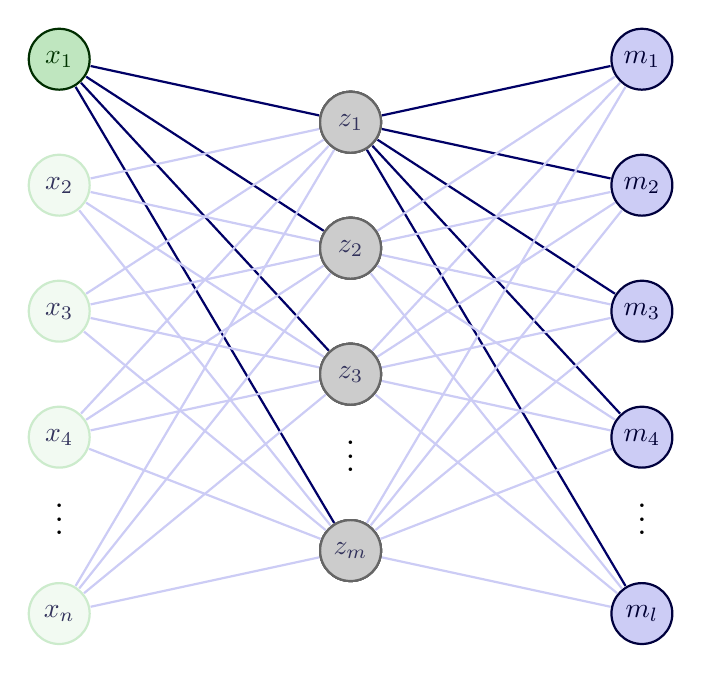
\begin{tikzpicture}
[x=3.7cm,y=1.6cm]
% BLOCK-SLOT  
      \def\NI{5} % number of nodes in input layers
      \def\NO{4} % number of nodes in output layers
      \def\NM{5} % number of nodes in M layers

      \def\yshift{0.4} % shift last node for dots

      % INPUT LAYER
      \foreach \i [evaluate={\c=int(\i==\NI); \y=\NI/2-\i-\c*\yshift; \index=(\i<\NI?int(\i):"n");}]
                  in {1,...,\NI}{ % loop over nodes
        \ifnum\i=1 % high-lighted node
            \node[node in,outer sep=0.6] (NI-\i) at (0,\y) {$x_{\index}$};
        \else
            \node[node,blue!20!black!80,draw=mygreen!20,fill=mygreen!5] (NI-\i) at (0,\y) {$x_{\index}$};
        \fi
      }
      % OUTPUT LAYER
      \foreach \i [evaluate={\c=int(\i==\NO); \y=\NO/2-\i-\c*\yshift; \indexi=(\i<\NO?int(\i):"m");}] in {\NO,...,1}{ % loop over nodes
              \foreach \j [evaluate={\indexK=(\j<\NI?int(\j):"n");}] in {1,...,\NI}{ % loop over nodes in previous layer
                    \node[node,blue!20!black!80,draw=black!60,fill=black!20]
                (NO-\i) at (1,\y) {$z_{\indexi}$};
            \ifnum\j=1 % high-lighted node
                \draw[connect,white,line width=1.2] (NI-\j) -- (NO-\i);
                \draw[connect] (NI-\j) -- (NO-\i);
                  node[pos=0.50] {\contour{white}{}};
            \else % other light-colored nodes
                % \draw[connect,white,line width=1.2] (NI-\j) -- (NO-\i);
                \draw[connect,myblue!20] (NI-\j) -- (NO-\i);
        \fi
        }
      }
        % INPUT LAYER
      \foreach \i [evaluate={\c=int(\i==\NI); \y=\NM/2-\i-\c*\yshift; \index=(\i<\NM?int(\i):"l");}]
                  in {1,...,\NM}{ % loop over nodes
          \node[node hidden](NM-\i) at (2,\y) {$m_{\index}$};
        }
      % OUTPUT LAYER
      \foreach \i [evaluate={\c=int(\i==\NM); \y=\NM/2-\i-\c*\yshift; \indexi=(\i<\NM?int(\i):"l");}] in {\NM,...,1}{ % loop over nodes
              \foreach \j [evaluate={\indexK=(\j<\NO?int(\j):"n");}] in {1,...,\NO}{ % loop over nodes in previous layer
                    % \node[node,blue!20!black!80,draw=black!60,fill=black!20]
                % (NO-\i) at (1,\y) {$z_{\indexi}$};
            \ifnum\j=1 % high-lighted node
                \draw[connect,white,line width=1.2] (NO-\j) -- (NM-\i);
                \draw[connect] (NO-\j) -- (NM-\i);
                  node[pos=0.50] {\contour{white}{}};
            \else % other light-colored nodes
                % \draw[connect,white,line width=1.2] (NI-\j) -- (NO-\i);
                \draw[connect,myblue!20] (NO-\j) -- (NM-\i);
        \fi
        }
      }
      
      % DOTS
      \path (NI-\NI) --++ (0,1+\yshift) node[midway,scale=1.2] {$\vdots$};
      \path (NO-\NO) --++ (0,1+\yshift) node[midway,scale=1.2] {$\vdots$};
      \path (NM-\NM) --++ (0,1+\yshift) node[midway,scale=1.2] {$\vdots$};

    \end{tikzpicture}
}

% The \icmltitle you define below is probably too long as a header.
% Therefore, a short form for the running title is supplied here:
\icmltitlerunning{Attention: Marginal Probabiliy is All You Need?}

\begin{document}

\twocolumn[
\icmltitle{Attention: Marginal Probability is All You Need?}

% It is OKAY to include author information, even for blind
% submissions: the style file will automatically remove it for you
% unless you've provided the [accepted] option to the icml2023
% package.

% List of affiliations: The first argument should be a (short)
% identifier you will use later to specify author affiliations
% Academic affiliations should list Department, University, City, Region, Country
% Industry affiliations should list Company, City, Region, Country

% You can specify symbols, otherwise they are numbered in order.
% Ideally, you should not use this facility. Affiliations will be numbered
% in order of appearance and this is the preferred way.
\icmlsetsymbol{equal}{*}

\begin{icmlauthorlist}
\icmlauthor{Ryan Singh}{sussex}
\icmlauthor{Christopher L. Buckley}{sussex}
% \icmlauthor{Firstname2 Lastname2}{equal,yyy,comp}
% \icmlauthor{Firstname3 Lastname3}{comp}
% \icmlauthor{Firstname4 Lastname4}{sch}
% \icmlauthor{Firstname5 Lastname5}{yyy}
% \icmlauthor{Firstname6 Lastname6}{sch,yyy,comp}
% \icmlauthor{Firstname7 Lastname7}{comp}
%\icmlauthor{}{sch}
% \icmlauthor{Firstname8 Lastname8}{sch}
% \icmlauthor{Firstname8 Lastname8}{yyy,comp}
%\icmlauthor{}{sch}
%\icmlauthor{}{sch}
\end{icmlauthorlist}

\icmlaffiliation{sussex}{School of Engineering and Informatics, University of Sussex}
% \icmlaffiliation{comp}{Company Name, Location, Country}
% \icmlaffiliation{sch}{School of ZZZ, Institute of WWW, Location, Country}

\icmlcorrespondingauthor{Ryan Singh}{rs773@sussex.ac.uk}
% \icmlcorrespondingauthor{Firstname2 Lastname2}{first2.last2@www.uk}

% You may provide any keywords that you
% find helpful for describing your paper; these are used to populate
% the "keywords" metadata in the PDF but will not be shown in the document
\icmlkeywords{Machine Learning, ICML}

\vskip 0.3in
]

% this must go after the closing bracket ] following \twocolumn[ ...

% This command actually creates the footnote in the first column
% listing the affiliations and the copyright notice.
% The command takes one argument, which is text to display at the start of the footnote.
% The \icmlEqualContribution command is standard text for equal contribution.
% Remove it (just {}) if you do not need this facility.

% \printAffiliations{}
\printAffiliationsAndNotice{}  % leave blank if no need to mention equal contribution
% \printAffiliationsAndNotice{\icmlEqualContribution} % otherwise use the standard text.

\begin{abstract}
Attention mechanisms are a central property of cognitive systems allowing them to selectively deploy cognitive resources in a flexible manner.   Attention has been long studied in the neurosciences and there are numerous phenomenological models that try to capture its core properties.  Recently attentional mechanisms have become a dominating architectural choice of machine learning and are the central innovation of Transformers.  The dominant intuition and formalism underlying their development has drawn on ideas of keys and queries in database management systems.  In this work, we propose an alternative Bayesian foundation for attentional mechanisms and show how this unifies different attentional architectures in machine learning. This formulation allows to to identify commonality across different attention ML architectures as well as suggest a bridge to those developed in neuroscience. 
% It also provides a description of a continuum between hard and soft attention in terms of the number of updates in a variational inference scheme.   
We hope this work will guide more sophisticated intuitions into the key properties of attention architectures as well suggest new ones. 
\end{abstract}

\section{Introduction}

Designing neural network architectures with favourable inductive biases lies behind many recent successes in Deep Learning \cite{baxter_model_2000}. In particular, the attention mechanism has  allowed language models to achieve human like generation abilities previously thought impossible \cite{vaswani_attention_2017}. The success of the attention mechanism as a domain agnostic architecture has prompted it to be adopted across a huge range of tasks and domains notably reaching state-of-the-art performance in visual reasoning and segmentation tasks \cite{dosovitskiy_image_2021, wang_image_2022}. 

Despite it's success, the role of the attention mechanism remains poorly understood. Indeed, it is unclear to what extent it relates to theories of cognitive attention which inspired it \cite{lindsay_attention_2020}. Here, we aim to provide a parsimonious description grounded in principles of probabilistic inference. This Bayesian perspective provides both a principled method for specifying prior beliefs and reasoning explicitly about the role of the attention variables. Further, understanding the fundamental computation permits us a unified description of different attention mechanisms in the literature. This proceeds in two parts.

% Numerous modifications to the attention mechanism have been made, either to improve the poor scaling $O(N^2)$ or for task-specific motivations.  
% It remains unclear, however, how to optimally design or analyse such modifications. Another often touted benefit of the attention mechanism is its interpretability.  In particular,  hard attention  maximises  interpretability by explicitly selecting individual features to attend to; an approach which is thought to better model  human-like attention.  Despite this, hard attention has not reached the same popularity as soft attention, which relies on probabilistic superpositions of input features, because its more difficult to train due to it's stochastic nature.

% Bayesian modelling, on the other hand,  provides both a principled method for specifying prior beliefs and reasoning explicitly about the role of the attention variables. Our approach combines the benefits of both by providing a link between the attention mechanism and Bayesian inference. 

% We aim to provide a unifying probabilistic account of different attention mechanisms in the literature. This proceeds in two parts. 

First, we show that `soft' attention mechanisms (e.g. self-attention, cross-attention, graph attention, which we call \textit{transformer attention} herafter) can be understood probabilistically as taking an expectation over possible connectivity structures, providing an interesting link between softmax-based attention and marginal likelihood.

Second, we extend the uncertainty over connectivity to a bayesian setting which, in turn, provides a theoretical grounding for iterative attention mechanisms (slot-attention, perciever and block-slot attention) \cite{locatello_object-centric_2020, singh_neural_2022, jaegle_perceiver_2021} and Modern Continuous Hopfield Networks \cite{ramsauer_hopfield_2021}. 

Additionally, we apply iterative attention to Predictive Coding Networks, 
 an influential theory in computational neuroscience, creating a new theoretical bridge between machine learning and cognitive science.

\begin{equation*}
    \begin{split}
        Attention(Q, K, V) &= \overbrace{softmax(\frac{QW_{Q}W_K^TK^T}{\sqrt{d_k}})}^\text{$p(E \mid Q, K)$}V \\
        &= \mathbb{E}_{p(E\mid Q, K)}[V]
    \end{split}
\end{equation*}

A key observation is that the attention matrix can be seen as the posterior distribution over an adjacency structure, $E$, and the full mechanism as computing an expectation of the value function $V(X)$ over the posterior beliefs about the possible relationships that exist between key and query.

This formalism provides an alternate Bayesian theoretical framing within which to understand attention models, which contrasts with the original framing in terms of  database management systems and data retrieval, providing a unifying framework to describe different attention architectures. Describing their difference only in terms of their edge relationships supporting more effective analysis and development of new architectures. Additionally providing  a principled understanding of the difference between hard and soft attention models.


\textbf{Contributions}
\begin{itemize}
    \item A unifying probabilistic framework for understanding attention mechanisms.
    \item We show self-attention and cross-attention can be seen as computing a marginal likelihood over possible network structures.  
    \item We show that slot-attention, block-slot-attention and modern continuous hopfield networks can all be seen as collapsed variational inference, where the possible network structures form the collapsed variables.
    \item Provide a bridge to Bayesian conceptions of attention from computational neuroscience, through the lens of Predictive Coding Networks.
    \item Provide a framework for reasoning about hard attention, and efficient approximations to the attention mechanism.

\end{itemize}


\section{Related Work}
\textbf{Attention as bi-level optimisation}
Mapping feed-forward architecture to a minimisation step on a related energy function has been called unfolded optimisation \cite{frecon_bregman_2022}. Taking this perspective can lead to insights about the inductive biases involved for each architecture. It has been shown that the cross-attention mechanism can be viewed as an optimisation step on the energy function of a form of Hopfield Network \cite{ramsauer_hopfield_2021}, providing a link between attention and associative memory. Whilst \cite{yang_transformers_2022} extend this view to account for self-attention. Our framework distinguishes hopfield attention, which does not allow an arbritary value matrix, from the standard attention mechanisms. Whilst there remains a strong theoretical connection, it  places the Hopfield Energy as an instance of variational free energy, aligning more closely with iterative attention mechanisms such as slot-attention. 

\textbf{Relationship to gaussian mixture model}
Previous works that have taken a probabilistic perspective on the attention mechanism note the connection to inference in a gaussian mixture model \cite{gabbur_probabilistic_2021, nguyen_improving_2022, ding_attention_2020}. Indeed \cite{annabi_relationship_2022} directly show the connection between the Hopfield energy and the variational free energy of a gaussian mixture model. Although gaussian mixture models, a special case of the framework we present here, are enough to explain cross attention they do not capture slot or self-attention. Further our framework allows us to extend the structural inductive biases beyond what can be expressed in a gaussian mixture model and capture the relationship to hard attention.

\textbf{Latent alignment and hard attention}
Several attempts have been made to combine the benefits of soft (differentiability) and hard attention. Most approaches proceed by sampling, e.g., using the REINFORCE estimator \cite{deng_latent_2018} or a $topK$ approximation \cite{shankar_surprisingly_2018}. The one most similar to ours embeds the full forward-backward algorithm within a forward pass \cite{kim_structured_2017}, our approach differs by offering a parsimonious description in terms of marginalisation over an implicit graphical model.

\textbf{Collapsed Inference}
Collapsed variational inference has most notably been employed in topic modelling \cite{teh_collapsed_2006}. To our knowledge, linking collapsed inference to attention in deep learning is completely novel.



\section{Transformer Attention} \label{neural-attention}
\subsubsection{Attention as Expectation}
We begin by demonstrating transformer attention is best seen as an expectation over latent variables. In the case of self and cross-attention, the expectation of a neural network with respect to possible adjacency structures.  

Let $x=(x_1,..,x_n)$ be observed variables, $\phi$ be some set of latent variables, and $y$ a variable we need to predict. Given a latent variable model $p(y, x , \phi) = p(y \mid x, \phi)p(x, \phi)$,  where $p(y\mid x, \phi)$ is parameterised by some function $v(y, x, \phi)$ e.g. a neural network. 

Our goal is to find $p(y\mid x)$, however $\phi$ are unobserved so we calculate the marginal likelihood.

$$p(y \mid x) = \sum_\phi p(\phi \mid x)v(y, x, \phi)$$
Importantly, the softmax function is a natural representation for the posterior 
\begin{equation*}
    p(\phi \mid x) = \frac{p(x, \phi)}{\sum_{\phi} p(x,\phi)} \label{marginalised}
\end{equation*}
\begin{equation*} 
    p(\phi \mid x) = softmax(\ln p(x, \phi))
\end{equation*}
Hence, transformer attention can be seen as weighting $v(x, \phi)$ by the posterior distribution $p(\phi \mid x)$. 
\begin{equation}
\begin{split}
    p(y \mid x) &= \sum_{\phi}softmax(\ln p(x, \phi))v(y, x, \phi) \\
    &=\mathbb{E}_{p(\phi \mid x)}[v(y, x, \phi)]\label{attention-is-expectation}
\end{split}
\end{equation}

We claim \eqref{attention-is-expectation} is exactly the equation underlying self and cross-attention. To make a more direct connection, we present the specific generative models corresponding to them. The latent variables $\phi$ are identified as possible \textit{relationships}, or edges, between each of the observed variables $x$ (keys and queries). 

A natural formalism for modelling these graphical relationships is Markov Random Fields.

\subsubsection{Pairwise Markov Random Fields}
Given a set of random variables $X = (X_v)_{v\in V}$ with probability distribution $[p]$ and a graph $G = (V, E)$. The variables form a pairwise Markov random field (MRF) with respect to $G$ if the joint density function $P(X=x)=p(x)$ factorises as follows
$$p(x) = \frac{1}{Z}\exp \left( \sum_{v \in V} \psi_v +  \sum_{e \in E} \psi_e \right)$$
where $Z$ is the partition function $\psi_{v}(x_v)$ and $\psi_e=\psi_{u,v}(x_u, x_v)$ are known as the node and edge potentials respectively\footnote{See \cite{shah_learning_2021} for a precise definition.}.

Beyond the typical set-up, we add a structural prior $p(E)$ over the adjacency structure of the underlying graph.
\begin{equation*}
\begin{split}
   p(x, E) &= P(x\mid E)P(E) \\ 
    &= \frac{1}{Z}{p(E)\exp \left(\sum_{v \in V} \psi_v +  \sum_{e \in E} \psi_e\right)}
\end{split}
\end{equation*}

We briefly remark that \eqref{attention-is-expectation}  respects factorisation of $[p]$ in the following sense; if the distribution admits a factorisation with respect to the latent variables $p(x, \phi)=\prod_i f_i(x, \phi_i)$ and $v(x, \phi) =  \sum_{i} v_i(x, \phi_i)$ then (applying the linearity of expectation) we may write 
\begin{equation}
    \mathbb{E}_{p(\phi \mid x)}[v(x, \phi)] = \sum_i\mathbb{E}_{p(\phi_i \mid x)}[v_i] \label{attention-expectation-independence}
\end{equation}
Permitting each factor to be marginalised independently.

In the case of an MRF, such a factorisation is natural. If the distibution over edges factorises into local distributions $p(E)= \prod_i p(E_i)$ (using independence properties of the MRF) we can write $p(x, E) = \frac{1}{Z}\prod_i f_i(x, E_i)$ where each $f_i =  P(E_i) \exp\sum_{v\in V}\psi_v{\sum_{e \in E_i}\psi_e}$ is itself an unnormalised MRF.

To recover cross-attention and self-attention are such models with we need only specify a structural prior and potential functions.
\begin{figure}
% \hfill
    \begin{subfigure}[t]{0.45\linewidth}
        \centering
        \resizebox{0.7\columnwidth}{!}{
            \crossattentiongraph
        }
        \caption{Cross Attention}
        \label{fig:cross-att}
    \end{subfigure}
    \begin{subfigure}[t]{0.45\linewidth}
    \centering
        \resizebox{\columnwidth}{!}{
            \selfattentiongraph
        }
        \caption{Self Attention}   
        \label{fig:self-att}
    \end{subfigure}


    \begin{subfigure}[c]{0.45\linewidth}
    \centering
        \resizebox{0.7\columnwidth}{!}{
            \mchngraph
        }
        \caption{Modern Continous Hopfield Network}   
        \label{fig:mchn}
    \end{subfigure}
    % \hfill
    \begin{subfigure}[d]{0.45\linewidth}
    \centering
        \resizebox{0.7\columnwidth}{!}{
            \slotattentiongraph
        }
        \caption{Slot Attention}   
        \label{fig:slot-att}
    \end{subfigure}
\label{fig:subfig1.a.4}

\caption{
    Comparison of different attention modules in the literature, the highlighted edges is representative of the marginalisation being performed for the random variable $E_1$, in \ref{fig:cross-att} and \ref{fig:self-att} all nodes are observed, as opposed to \ref{fig:mchn} and \ref{fig:slot-att}, where there are latent nodes (indicated in grey).
}
\label{fig:my_label}
\end{figure}



\subsubsection{Cross Attention}
\begin{itemize}
    \item Key nodes  $K =(x_1,..,x_n)$
    \item Query nodes $Q = (x_1',...,x_m')$
    \item Structural prior $p(E) = \prod_{i=1}^m p(E_i)$, where $E_i \sim Uniform\{(x_1, x_i'),..,(x_n, x_i')\}$, such that each query node is uniformly likely to connect to each key node.
    \item Edge potentials $\psi(x_j, x_i')=x_i'^TW_{Q}^TW_{K}x_j$, in effect measuring the similarity of $x_j$ and $x_i'$ under a certain transformation.
    \item Value function $V_i(K, Q, E_i) = W_V x_{s(E_i)}$, a linear transformation applied to the node, $x_{s(E_i)}$, the start of the edge $E_i$.
\end{itemize}
Taking the posterior expectation in each of the factors defined in two \eqref{attention-expectation-independence} gives the standard cross- attention mechanism
$$\mathbb{E}_{p(E_i\mid Q, K)}[V_i] =  \sum_{j} softmax_j(x_i'^TW_{Q}^TW_{K}x_j)W_{V} x_j$$
$$\mathbb{E}_{p(E\mid Q, K)}[V] =  softmax(Q^TW_Q^TQ_KK)W_VK$$

\subsubsection{Self Attention}
\begin{itemize}
    \item Nodes  $K = Q = (x_1,..,x_n)$
    \item Structural prior $p(E) = \prod_{i=1}^n p(E_i^{\rightarrow})$, where $E_i^{\rightarrow} \sim Uniform\{(x_1, x_i),..,(x_n, x_i)\}$, such that each node is uniformly likely to connect to every other node.
    \item Edge potentials $\psi(k_j, k_i)=x_i^TW_{Q}^TW_{K}x_j$, in effect measuring the similarity of $x_j$ and $x_i'$ under a certain transformation.
    \item Value function $V_i(K, Q, E_i) = W_V x_{s(E_i)}$, a linear transformation applied to the node, $x_{s(E_i)}$, the start of the edge $E_i$.
\end{itemize}
Again, taking the posterior expectation in each of the factors defined in two \eqref{attention-expectation-independence} gives the standard self- attention mechanism
$$\mathbb{E}_{p(E_i\mid Q, K)}[V_i] =  \sum_{j} softmax_j(x_i^TW_{Q}^TW_{K}x_j)W_{V} x_j$$
$$\mathbb{E}_{p(E\mid Q, K)}[V] =  softmax(K^TW_Q^TW_KK)W_VK$$


\section{Iterative Attention}
We continue by extending attention to full Bayesian inference. In essence applying the attention trick, marginalisation of attention variables, to the variational free energy (a.k.a the ELBO).

Modern Continuous Hopfield Networks can be seen as a particular instance of this class of system, allowing us to reproduce the `hopfield attention' updates of \cite{ramsauer_hopfield_2021} within a probabilistic context. Under different structural priors we  recover other iterative attention models; slot-attention \cite{locatello_object-centric_2020}, block-slot attention \cite{singh_neural_2022} and Perciever \cite{jaegle_perceiver_2021}. Further, we showcase a specific advantage of bayesian attention, hard attention.



\subsubsection{Collapsed Inference}
We present a version of collapsed variational inference \cite{teh_collapsed_2006} showing how this results in a bayesian attention mechanism. The term attention mechanism is apt due to the surprising similarity in form between the variational updates \eqref{expected_attention} and neural attention mechanism \eqref{attention-is-expectation}. 

Our setting is the latent variable model $p(x,z, \phi)$, where $x$ are observed variables, and $z$, $\phi$, are latent variables. Typically  we wish to infer $z$ given $x$. 

Collapsed inference proceeds by marginalising out the extraneous latent variables $\phi$
\begin{equation}
    p(x, z) = \sum_{\phi} p(x,z, \phi) \label{marginalised}
\end{equation}

We define a recognition density $q(z) \sim N(z; \mu)$ and optimise the variational free energy with respect to the parameters, $\mu$, of this distribution.
$$\min_{\mu} F(x, \mu) = \mathbb{E}_q[\ln q_\mu(z) - \ln p(x,z)]$$
Under a typical  Laplace approximation, we can write the variational free energy as  $F \approx -\ln p(x, \mu)$ \footnote{See appendix for a more principled derivation taking account of higher order terms}.  Substituting in \eqref{marginalised} and taking the derivative with respect to the variational parameters yields,
$$F(x, \mu) = - \ln \sum_{\phi} p(x, \mu, \phi)$$
\begin{equation}
    \frac{\partial F}{\partial \mu} = - \frac{1}{\sum_{\phi} p(x, \mu, \phi)}\sum_{\phi} \frac{\partial}{\partial \mu}p(x, \mu, \phi) \label{general_attention}
\end{equation}

Which connects bayesian attention with the standard attention \eqref{attention-is-expectation}. To clarify this, we employ the log-derivative trick, substituting $p_\theta = e^{\ln p_\theta}$ and re-express \eqref{general_attention} in two ways:
\begin{equation}
    \frac{\partial F}{\partial \mu} = -\sum_{\phi} softmax_{\phi}(\ln p(x, \mu, \phi))\frac{\partial}{\partial \mu}\ln p(x, \mu, \phi) \label{softmax_derivative}
\end{equation}
\begin{equation}
    \frac{\partial F}{\partial \mu} = \mathbb{E}_{p(\phi \mid x, \mu)}[-\frac{\partial}{\partial \mu}\ln p(x, \mu, \phi)] \label{expected_attention}
\end{equation}

%alternate para
The first form reveals the softmax which is ubiquitous in all attention models. The second, suggests the variational update should be evaluated as the expectation of the  typical variational gradient (the term within the square brackets) with respect to the posterior over the parameters represented by the random variable $\phi$. 

In other words, bayesian attention is exactly the nueral attention mechanism applied iteratively, where the value function is the variational free energy gradient. We derive updates for a general MRF before again recovering (iterative) attention models in the literature  by specifying particular distributions. 


\subsubsection{Free Energy of a marginalised MRF}

Recall the factorised MRF, $p(E)= \prod_i p(E_i)$.  $p(x, E) = \frac{1}{Z} \prod_i f_i(x, E_i)$ with each $f_i =  P(E_i)\exp\sum_{v\in V}\psi_v{\sum_{e \in E_i}\psi_e}$. Independence properties mean the  marginalisation necessary for collapsed inference can be simplified

\begin{equation*}
        \sum_E p(x, E) = \frac{1}{Z}\prod_i \sum_{E_i} f_i(x, E_i)
\end{equation*}

In an inference setting the nodes are partitioned into observed nodes, $x$, and latent nodes, $z$. The variational free energy \eqref{general_attention} and the associated forms of it's derivative can be expressed  
\begin{equation*}  
    F(x, \mu, \theta) = - \sum_i\ln \sum_{E_i} f_i(x, \mu, E_i) 
\end{equation*}
$$\frac{\partial F}{\partial \mu_j} =  -\sum_i \sum_{E_i} softmax(f_i(x, \mu, E_i))\frac{\partial f_i}{\partial \mu_j}$$


Similar to hard attention approaches, the random variable $E$  is an explicit alignment variable. However, unlike hard attention, we avoid inferring $E$ \textit{explicitly} using the collapsed inference approach outlined above. 


\subsubsection{Quadratic Potentials and the convex concave procedure}
We follow \cite{ramsauer_hopfield_2021} in using the CCCP to derive a fixed point equation, which necessarily reduces the free energy. 

Assuming the node potentials are quadratic $\psi(x_i) = -\frac{1}{2}x_i^2$ and the edge potentials have the form $\psi(x_i, x_j) = x_iWx_j$.
\begin{equation}
    \mu_j^{*} =  \sum_i \sum_{E_i} softmax(g_i(x, \mu, E_i))\frac{\partial g_i}{\partial \mu_j} \label{fixed_point_attention}
\end{equation}
Where $g_i = \sum_{e \in E_i}\psi_e$.

By way of the CCCP \cite{yuille_concave-convex_2001}, this fixed point equation has the property $F(x, \mu_j^*, \theta) \leq F(x, \mu_j, \theta)$ with equality if and only if $\mu_j^*$ is a stationary point of $F$.

We follow the \ref{neural-attention} in specifying specific structural priors and potential functions to recover different iterative attention mechanisms.

\subsubsection{Hopfield-Style Cross Attention}
Let the observed $x =(x_1,..,x_n)$ and latent nodes $z=(z_1,..,z_m)$ have the following structural prior $p(E) = \prod_{i=1}^m p(E_i)$, where $E_i \sim Uniform\{(x_1, z_i),..,(x_n, z_i)\}$. And define edge potentials $\psi(x_j, z_i)=z_iQ^TKx_j$, Application of \eqref{fixed_point_attention}
$$\mu_i^{*} =  \sum_{j} softmax_j(\mu_iW_{Q}^TW_Kx_j)W_Q^T W_K x_j$$

When $\mu_i$ is initialised to some query $\xi$ the system
\cite{ramsauer_hopfield_2021} the fixed point update is given by $\mu_i^{*}(\xi) = \mathbb{E}_{p(E_i \mid x, \xi)}[W_Q^T W_Kx_{t(E_i)}]$. When the patterns $x$ are well separated, $\mu_i^*(\xi) \approx W_Q^T W_Kx_j$, where $W_Q^T W_Kx_j$ is the closest vector and hence can be used as an associative memory.

\subsubsection{Slot Attention}
Slot attention \cite{locatello_object-centric_2020} is an object centric learning module built on top of an iterative attention mechanism. Here we show this is a simple adjustment of the prior beliefs on our edge set.

With the same set of nodes and potentials, replace the prior over edges with 
$p(E) = \prod_{j=1}^n p(E_j)$, $E_j \sim Uniform\{(x_j, z_1),..,(x_j, z_m)\}$
\begin{equation*}
    \mu_i^{*} =  \sum_{j} softmax_i(\mu_iQ^TKx_j)Q^T K x_j
\end{equation*}

Whilst the original slot attention employed an RNN to aid the basic update shown here, the important feature is that the softmax is taken over the `slots', $\mu$. This forces competition between slots to account for the observed variables, forcing object centric representations. For example, if the observed variables $x$ are image patches, the slots are forced to cluster similar patches together in order increase the overall likelihood of said patches. The word cluster is accurate, in fact there is an exact equivalence between this mechanism and a step of EM on a gaussian mixture model.

% \subsubsection{Self Attention} \label{self-attention}
% Self attention is functionally the same as cross-attention, except the queries and keys are projections of the data \cite{vaswani_attention_2017}. One way to view this, within the variational inference framework we present, is that $\mu_j = Qx_j$ is an amortisation. Specifically, self attention applies a hybrid approach to inference \cite{tschantz_hybrid_2022}, first the variational parameters are calculated using global parameters $Q$ followed by one step of iterative inference. Hence
% $$\mu_i^{*} =  \sum_{j} softmax_j(x_iQ^TKx_j)K x_j$$
% Inference is performed in the forward pass, and the amortised parameter $Q$ is adjusted in the backward pass, in order to better approximate the inference.

% This perspective reframes the function of self-attention as inference about the latent states that are most likely, given the observed sequence, under a probabilistic model that has learnt over multiple examples. 

\subsubsection{Block Slot Attention}
\cite{singh_neural_2022} suggest combining an associative memory ability with an object-centric slot-like ability and provide an iterative scheme for doing so, alternating between slot-attention and hopfield updates. 

Our framework permits us to flexibly combine different attention mechanisms through different latent graph structures, allowing us to derive a model informed version of block-slot attention. In this setting we have three sets of variables $X$, the observations, $Z$ the latent variables to be inferred and $M$ which are parameters.

Define the pairwise MRF $X = \{x_1,...,x_n\}$, $Z = \{z_1,...,z_m\}$ and $M = \{m_1,...,m_l\}$ with a prior over edges  $p(E) = \prod_{j=1}^m p(E_j)\prod_{k=1}^l p(\Tilde{E_k})$, $E_j \sim Uniform\{(x_j, z_1),..,(x_j, z_m)\}$, $\Tilde{E_k} \sim Uniform\{(z_1, m_k),..,(z_m, m_k)\}$, with edge potentials between $X$ and $Z$ given by $\psi(x_j, z_i)=z_iQ^TKx_j$ and between $Z$ and $M$, $\psi(z_i, m_k)=z_i \cdot m_k$

applying \eqref{fixed_point_attention} gives
\begin{equation*}
    \begin{split}
        \mu_i^{*} =  &\sum_{j} softmax_i(\mu_iQ^TKx_j)Q^T K x_j \\
                    & + \sum_{k} softmax_k(\mu_i \cdot m_k)m_k
    \end{split}
\end{equation*}

\begin{figure}
    \centering
        \resizebox{0.7\columnwidth}{!}{
        \blockslotattentiongraph
        }
    \caption{Block Slot Attention}
    \label{fig:my_label}
\end{figure}

In the original block-slot attention each slot $z_i$ is broken into blocks, where each block can access block-specific memories i.e. $z_i^{(b)}$ can has possible connections to memory nodes $\{m_k^{(b)}\}_{k\leq l}$. Allowing objects to be represented by slots which in turn disentangle features of each object in different blocks. We presented a single block version above, however it is easy to see that the update extends to the multiple block version 
applying \eqref{fixed_point_attention} gives
\begin{equation*}
    \begin{split}
        \mu_i^{*} =  &\sum_{j} softmax_i(\mu_iQ^TKx_j)Q^T K x_j \\
                    & + \sum_{k, b} softmax_k(\mu_i^{(b)} \cdot m_k^{(b)})m_k^{(b)}
    \end{split}
\end{equation*}


\section{Predictive Coding Networks}

Predictive Coding Networks (PCN) have emerged as an influential theory in computational neuroscience \cite{rao_predictive_1999, friston_predictive_2009, buckley_free_2017}. Building on theories of perception as inference and the Bayesian brain, PCNs perform approximate Bayesian inference by minimising the variational free energy which is manifested in the minimisation of local prediction errors. The continuous time dynamics at an individual neuron are given by
$$
    \frac{\partial \mathcal{F}}{\partial \mu_i} = -\sum_{\phi^{-}} k_{\phi}\epsilon_{\phi} + \sum_{\phi^{+}}k_{\phi}\epsilon_{\phi}w_{\phi}
$$
Where $\epsilon$ are prediction errors, $w$ represent synaptic strength and $k$ are node specific precisions representing uncertainty in the generative model \cite{millidge_theoretical_2022}.

A natural extension is to apply collapsed inference over the set of incoming and out going connection, i.e. a locally factorised prior over possible connectivity. In the notation of the previous section, we have an MRF with a hierarchical structure $Z = \{Z^{(0)}, ..., Z^{(l)}, ..., Z^{(N)} \}$ where the prior on edges factorises into layerwise $p(E^{(l)})=\{(z_i, z_j): (z_i, z_j) \in Z^{(l-1)}\times Z^{(l)}\}$ and potential functions $\phi(z_i, z_j)=\epsilon_{i,j}^2 = k_{j}(z_j - w_{i,j}z_i)^2$.
% $$
%     \frac{\partial \mathcal{F}}{\partial \mu_i} = -\sum_{\phi^{-}} softmax( {-\epsilon_\phi}^2)k_{\phi}\epsilon_{\phi} + \sum_{\phi^{+}} softmax( {-\epsilon_\phi}^2)k_{\phi}\epsilon_{\phi}w_{\phi}
% $$
\begin{equation*}
    \begin{split}
          \frac{\partial \mathcal{F}}{\partial \mu_i} =  &-\sum_{\phi^{-}} softmax( {-\epsilon_\phi}^2)k_{\phi}\epsilon_{\phi} \\
                    & + \sum_{\phi^{+}} softmax( {-\epsilon_\phi}^2)k_{\phi}\epsilon_{\phi}w_{\phi}
    \end{split}
\end{equation*}

The resulting dynamics induce a ``normalisation" across prediction errors received by a neuron through the softmax function. This dovetails nicely with theories of attention as normalisation in psychology and neuroscience. In contrast previous predictive coding based theories of attention have focused on the precision terms, $k$, due to their ability to up and down regulate the impact of prediction errors \cite{feldman_attention_2010}. Here we see the softmax term can also perform this regulation, while also exhibiting the fast winner-takes-all dynamics that are associated with cognitive attention.


\subsection{Discussion}

In this section we will briefly discuss what can be gained from looking at the attention mechanism as a problem of inference.


\subsubsection{Hard Attention}

% We present how notions of soft and hard attention relate to our framing of neural and bayesian attention.

Recall \eqref{attention-is-expectation} neural attention may be viewed as calculating an expectation over latent variables $\mathbb{E}_{p(\phi \mid x)}[v(x, \phi)]$. Here the mechanism is `soft' because we weight multiple possibilities of attention variable $\phi$. Hard attention, on the other hand, proceeds with a single sample from $p(\phi \mid x)$. It has been argued this is more biological, more interpretable and has lower computational complexity. Previously the inferior performance of hard-attention has been attributed to it's hard to train, stochastic nature. However, our framing of soft attention as exact marginalisation offers an alternate explanation. Stochastic approximations (hard attention) will always suffer compared with exact marginalisation (soft attention). Further our framework provides a method for seamlessly interchanging hard and soft-attention. Since the distribution $p(\phi \mid x)$ a the categorical distribution, at any point (during training or inference) it is possible to implement hard attention by taking a single sample $\phi^*$ from $p(\phi \mid x)$ yielding $v(x, \phi^*)$. 

There are two issues with this approach to collapsing the attention distribution. First, the single sample will collapse any uncertainty, secondly calculation of $p(\phi \mid x)$, in order to sample, still incurs a quadratic penalty $O(n^2)$. However we can employ tools from probability theory to help us analyse the cost of sampling, and linear approximations to the attention distribution.



\subsubsection{Efficient Transformers}

Consider some distribution $q$ attempting to approximate $p(\phi \mid x)$ we can quantify the information loss with the relative entropy 
$$\mathcal{L}[p,q] \triangleq D_{KL}[q(\phi) \mid \mid p(\phi \mid x)] = H[q] + \mathbb{E}_q[p(\phi \mid x)]$$
In the hard attention approximation a single sample from $p$ is used as an approximation $\mathcal{L}[p,q] = -\ln p(\phi^* \mid x)$ and perhaps intuitively $\mathbb{E}[\mathcal{L}] = H[p]$ i.e. hard attention is a good approximation when the attention distribution is low-entropy which can be controlled by the temperature parameter (Appendix \ref{Temperature}).

Many of the efficient alternatives to attention, such as low-rank and linear approximations, can be cast as approximating $p(\phi \mid x)$ with $q(\phi \mid x)$ where calculating $q$ is less expensive than exact marginalisation. Estimating $\mathcal{L}$ could be used to quantify the relative information loss when using these alternatives. Another direction taken to reduce computational complexity of the attention mechanism is sparsification the attention matrix, which in our framework reduces to adjustments to the prior over edges (Appendix \ref{positional-encodings}).

\subsubsection{New Designs}

The main difference between the description presented and previous probabilistic descriptions is to view soft attention as a principled, exact, probabilistic calculation, with respect to an implicit probabilistic model, as opposed to an impoverished approximation. This leads to possibility of designing new attention mechanisms by altering the distribution that the mechanism marginalises over, either by adjusting the structural prior, or the potential functions. We hope this will enable new architectures to be designed in a principled manner. 


% A hard attention mechanism would be $v(x, \phi^{MAP})$, however this function, $\phi^{MAP} = \arg \max_{\phi} p(\phi\mid x)$, is not differentiable.

% However we can see the attention scheme above as an EM descent on the free energy of the full inference problem
% \begin{equation}
%     \begin{split}
%         \Tilde{F} &= \mathbb{E}_q[\ln q(\phi, x , z) - \ln p(\phi, x, z)] \\
%                 &= \mathbb{E}_{q(z)}[D_{KL}[q(\phi \mid x, z) \mid \mid p(\phi \mid x, z)]] \\
%                 & + \mathbb{E}_q[\ln q(z \mid x) - \ln p(x, z)] \\
%     \end{split}
% \end{equation}
% \begin{equation}
%     F \approx D_{KL}[q(\phi \mid x, \mu) \mid \mid p(\phi \mid x, \mu)] - \ln p(x, \mu)
% \end{equation}

% Where the last equation again employed the laplace approximation. Consider the update $q^{(t)} \rightarrow q^{(t+1)}$ in two stages. An E step which sets $q^{(t+1)}(\phi \mid \mu, x) = p(\phi \mid \mu, x)$, this necessarily minimises the first term. Then an M step, in which variational parameters $\mu$ are updated to optimise the second term. 





% In the unusual situation where you want a paper to appear in the
% references without citing it in the main text, use \nocite
\bibliography{main}
\bibliographystyle{icml2023}


%%%%%%%%%%%%%%%%%%%%%%%%%%%%%%%%%%%%%%%%%%%%%%%%%%%%%%%%%%%%%%%%%%%%%%%%%%%%%%%
%%%%%%%%%%%%%%%%%%%%%%%%%%%%%%%%%%%%%%%%%%%%%%%%%%%%%%%%%%%%%%%%%%%%%%%%%%%%%%%
% APPENDIX
%%%%%%%%%%%%%%%%%%%%%%%%%%%%%%%%%%%%%%%%%%%%%%%%%%%%%%%%%%%%%%%%%%%%%%%%%%%%%%%
%%%%%%%%%%%%%%%%%%%%%%%%%%%%%%%%%%%%%%%%%%%%%%%%%%%%%%%%%%%%%%%%%%%%%%%%%%%%%%%
\newpage
\appendix
\onecolumn
% \section{Neural Attention Relationship to EM}
% As in section \ref{neural-attention}, we have a model specified by $p_{\theta}(y, x, \phi) = p_{\theta}(y \mid x, \phi)p_{\theta}(\phi, x)$. Given training pair $\{(x, y)\}$, our goal is $$\max_{\theta}p_{\theta}(y \mid x)$$
% However we are missing latent variable information, we can formulate this optimisation as expectation maximisation. Consider

% \begin{equation*}
%     \begin{split}
%         \ln p(y \mid x; \theta) &= \mathbb{E}_{p(\phi \mid x; \theta')}[\ln p(y, \mid \phi, x; \theta)] + \mathbb{E}_{p(\phi \mid x; \theta')}[\ln p(\phi \mid x; \theta)] - \mathbb{E}_{p(\phi \mid x; \theta')}[\ln p(\phi \mid y, x; \theta)] \\
%         &= Q(\theta \mid \theta') + H(\theta \mid \theta')
%     \end{split}
% \end{equation*}

% E Step: Calculate $Q(\theta \mid \theta') = \mathbb{E}_{p(\phi \mid x; \theta')}[\ln p(y  \mid \phi, x; \theta)] = Attention$

% M step: Minimise $Q(\theta \mid \theta')$ w.r.t $\theta$

% For proof of convergence we just need to show $H(\theta \mid \theta') \geq H(\theta' \mid \theta')$

% \section{Derivation of Collapsed Inference}
% \begin{lemma}
% Let $s_{\phi} = softmax(\ln p(x,\phi))$. Then the following identity holds $- \ln \sum_{\phi} p(x, \phi) = -\sum s_\phi \ln p(x, \phi) + \sum_\phi s_\phi\ln s_\phi$
% \end{lemma}
% \begin{proof}
% This identity follows from the fact that $q = s_\phi = p(\phi \mid x)$ attains the minimum of the following variational free energy
% $F[p, q] = \mathbb{E}_{q}[-\ln p(x, \phi)] + H[q]$
% \end{proof}

% We can now justify our perspective on collapsed inference without invoking the laplace assumption. 

% Consider the  free energy
% $$
% F[\phi, q] = \mathbb{E}_{q(z; \mu)q(\phi;\hat{\phi})}[- \ln p(x,z, \phi)] + H[q_\mu] + H[q_\phi] 
% $$
% We can perform co-ordinate descent, by alternating minimising 
% the objective with respect to variational parameters $q(z; \mu)$ and $\phi$. We first assume a set of parameters $\mu_t$
% Then
% $$
% F[\phi, q] = \mathbb{E}_{q(z; \mu)q(\phi;\hat{\phi})}[- \ln p(x, \phi \mid z) + \ln p(z)] + H[q_\mu] + H[q_\phi] 
% $$
% Which as we have shown above is exactly minimised when $q_\phi = p(\phi \mid x, \mu_{t})$ and the identity holds, hence we can collapse the expectation with respect to $q_{\phi_t}$
% $$
% F[\phi, q] = \mathbb{E}_{q(z; \mu)}[- \sum s_\phi \ln p(x, z, \phi) + \ln p(z)] + H[q_\mu] + H[q_\phi] 
% $$
% Now for since $\phi$ is not dependent on $z$ we can move the expectation inside
% $$
% F[\phi, q] = \sum s_\phi \mathbb{E}_{q(z; \mu)}[- \ln p(x, z, \phi) + \ln p(z)] + H[q_\mu] + H[q_\phi] 
% $$

% \section{Positional Encodings} \label{positional-encodings}

% Attention mechanisms are usually used in combination with some form of positional encoding strategy, since the mechanism itself is position agnostic. Multiple encodings have been suggested, including relative, absolute and rotational encodings, further multiple works have demonstrated the benefit of learnable position encodings. 

% In a bayesian scheme, the natural way of encoding such inductive biases is through the prior, and learn-ability amounts to letting the prior be data-driven. We use our framework to derive a principled derivation of learnable position encodings, which provides insight into the currently available strategies.

% In the setting of self-attention, \ref{self-attention}, if the prior over edges is categorical i.e. $P(E_i = \{(x_j, z_i)\}) = p_{i,j}$, it can be fully specified by the matrix $(P)_{i,j} = p_{i,j}$. This leads to the modified attention update
% $$\mu_i^{*} =  \sum_{j} softmax_j(x_iQ^TKx_j + \ln p_{ij}) x_j$$

% However this requires local parameters for each node $z_i$. A more natural prior assign a different probability to the relative distance of $i$ from $j$. This is achieved with $P = circ(p_1, p_2,..,p_n)$, where $circ$ is the circulant matrix of $(p)_{i\leq n}$. Due to properties of circulant matrices $\ln P_{ij}$ can be reparameterised with the hartley transform
% $$\ln P_{i,j} = \sum_k \beta_k [cos(k \theta_{i,j}) + sin(k \theta_{i,j})] = \beta \cdot b^{(i,j)}$$
% Where $b^{(i,j)}_k = cos(k \frac{i - j}{2\pi n}) + sin(k \frac{i - j}{2\pi n})$ can be thought of as a relative position encoding, and $\beta$ are parameters to be learnt.
% $$\mu_i^{*} =  \sum_{j} softmax_j(x_iQ^TKx_j + \beta \cdot b^{(i,j)})K x_j$$

% \section{Convolution}

% A convolutional layer is given by the following transformation
% $$C(X)_i = \sum_{j \in K} X_{i+j}W_j$$
% Where $K$ is size of the kernel, and $W$ is a kernel to be learnt.

% \begin{itemize}
%     \item Data nodes  $X =(x_1,..,x_n)$
%     \item Kernel nodes $Q = (c_1,...,c_N)$
%     \item Structural prior $p(E_i)$ where $E_i \sim Uniform\{(c_j, x_{i+j}): j \in K\}$
%     \item Trivial edge potentials $\phi(z_i, x_j)=0$
%     \item Value function $V_i = W_{E_i} X_{t(E_i)}$
% \end{itemize}

% This system yields the standard convolution
% $$\mathbb{E}_{p(E_i\mid Q, K)}[V_i] =  \sum_{j\in K} X_{i+j}W_{j} $$

% We remark also it becomes clear a transformer can express a convolution as shown by \cite{}. Since clearly the system above is contained within the self-attention model, with a specific position encoding prior (that is 1 for relative position sizes within the kernel, 0 otherwise). The only subtlety, is $W_{E_i}$ usually being a fixed matrix (not dependent on $E_i$) in standard attention, hence the authors show multiple heads can do each part of the computation.


% \section{Classification}

% \begin{itemize}
%     \item Data node  $x$
%     \item Target nodes $Y = (e_1,...,e_m)$, where $e_i$ is a standard basis vector
%     \item Structural prior where $E \sim Uniform\{(x, e_1),..,(x, e_n)\}$
%     \item Edge potentials $\phi(x, e_i)=f_\theta(x) \cdot e_i$, where $f_\theta$ is some function, e.g. a neural network
%     \item Value function $V(x, Y, E) = e_i$
% \end{itemize}
% Taking the posterior expectation yield the softmax layer widely used for classification
% $$\mathbb{E}_{p(E\mid X, y)}[V] =  \sum_{j} softmax_j(f_\theta(x)[j])e_j = softmax_j(f_\theta(x)[j])$$
% This fact that underlying classifiers there is an implicit generative model was reported by \cite{grathwohl_your_2020}.

% \section{Temperature} \label{Temperature}


% This approach is similar in form and function to the relative encodings suggested by \cite{huang} and \cite{shaw}. We hypthosise the original absolute encodings  \cite{vaswani_attention_2017} are perhaps also computing this transform. Consider the attention score between position $i$ and $j$, with positional embeddings $p_i$ and $p_j$. $(x_i + pos_i)^TK^TQ(x_j + pos_j) = x_i^TK^TQx_j + pos_i^TK^TQpos_j$. Consdering the second (positional) term only
% \begin{equation*}
%     pos_i^TK^TQpos_j = \sum_{k=1}^{d_{model} / 2}\sum_{m=1}^{d_{model /2 }}   \gamma_{k,m} cos(\frac{i}{D_k} - \frac{j}{D_m})
% \end{equation*}
% Where $D_k=10000^{2k/d_{model}}$, and the 


% \subsubsection{Classification and Convolution}


% \subsubsection{Bilevel Optimisation}
% The unfolded optimisation perspective proposes that if we can find a correspondence between a forward pass in a neural network and an optimisation step on an energy function, we can view neural network as a two-level optimisation process. A forward pass computes the first level, whilst the backwards pass computes the second level.
% $$\mu^*(\theta, x) = \arg \min_\mu F(\mu, \theta, x)$$ 
% $$\theta^* = \arg \min_\theta l(\psi(\mu^*(\theta, x)), y)$$
% Where $x$ is the input to the network, $y \in \mathbb{R}^{m}$ is a desired output $l(y, y')$ is some loss function, $\psi:\mathbb{R}^N \rightarrow \mathbb{R}^M$ is some transformation.

% In our case the energy function is a variational free energy, meaning the forward pass can be interpreted as approximate inference and the backwards pass adjusts the parameters of the model in order to satisfy the meta-objective $l(y, y')$. i.e. we learn a probabilistic model that is useful for the downstream task in question.
% \section{You \emph{can} have an appendix here.}

% You can have as much text here as you want. The main body must be at most $8$ pages long.
% For the final version, one more page can be added.
% If you want, you can use an appendix like this one, even using the one-column format.
%%%%%%%%%%%%%%%%%%%%%%%%%%%%%%%%%%%%%%%%%%%%%%%%%%%%%%%%%%%%%%%%%%%%%%%%%%%%%%%
%%%%%%%%%%%%%%%%%%%%%%%%%%%%%%%%%%%%%%%%%%%%%%%%%%%%%%%%%%%%%%%%%%%%%%%%%%%%%%%


\end{document}


% This document was modified from the file originally made available by
% Pat Langley and Andrea Danyluk for ICML-2K. This version was created
% by Iain Murray in 2018, and modified by Alexandre Bouchard in
% 2019 and 2021 and by Csaba Szepesvari, Gang Niu and Sivan Sabato in 2022.
% Modified again in 2023 by Sivan Sabato and Jonathan Scarlett.
% Previous contributors include Dan Roy, Lise Getoor and Tobias
% Scheffer, which was slightly modified from the 2010 version by
% Thorsten Joachims & Johannes Fuernkranz, slightly modified from the
% 2009 version by Kiri Wagstaff and Sam Roweis's 2008 version, which is
% slightly modified from Prasad Tadepalli's 2007 version which is a
% lightly changed version of the previous year's version by Andrew
% Moore, which was in turn edited from those of Kristian Kersting and
% Codrina Lauth. Alex Smola contributed to the algorithmic style files.
